\chapter{Graphs and Tree}



\section{Trees}


\subsection{Heavy Light Decomposition}

\subsubsection{Motivating Problem}

Given a Tree, handle the following queries:
\begin{itemize}
  \item Update(edge, weight): Change the weight of any given edge in the Tree.
  \item Query(nodeX, nodeY): Find the heaviest eadge between two nodes, x and y.
\end{itemize}

\begin{figure}[h]
  \begin{center}
    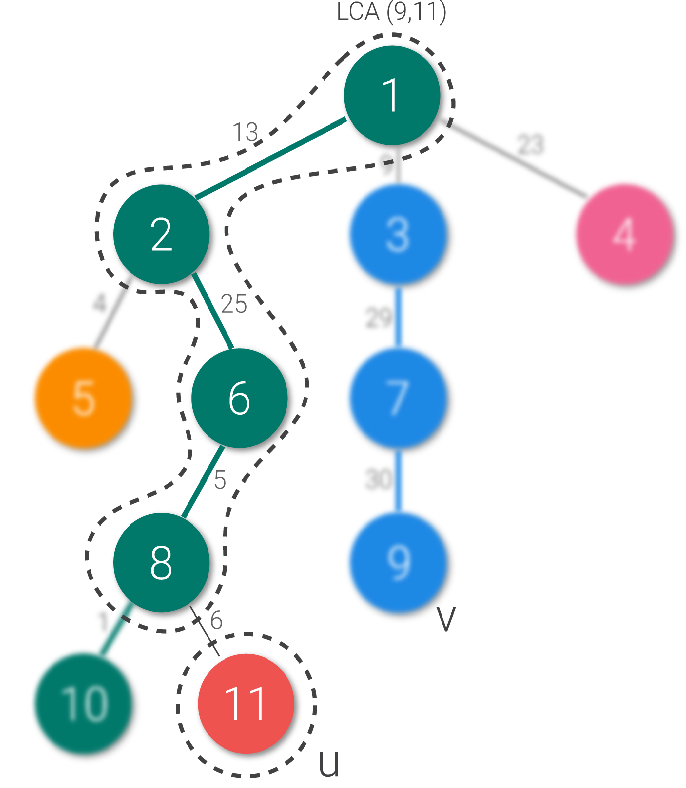
\includegraphics[scale=0.2]{img/heavy-light-decomposition.png}
  \end{center}
  \caption{Heavy Light decomposition of a Tree}
\end{figure}


\section{Basic Algorithms on Graphs}


\subsection{List of algorithms}

\begin{itemize}
  \item Depth First Search
  \item Breadth First Search
  \item Shortest Path - Dijkstra's
  \item Shortest Path - Bellman Ford
  \item Shortest Path - Floyd Warshall
  \item Connected Components
  \item Topological Sort
  \item Prim's Maximum Spanning Tree

\end{itemize}


\subsection{Code}

\lstinputlisting[basicstyle=Large,style=cpp]{code/Graphs.hpp}